% Fronteirs template Version 2.4 Generated 2014/03/12 %%%
\documentclass{frontiersSCNS} % for Science articles

%\setcitestyle{square}
\usepackage{url,lineno}
\usepackage[english]{babel}
\linenumbers

\copyrightyear{}
\pubyear{}

\def\journal{Genetics}%%% write here for which journal %%%
\def\DOI{} \def\articleType{Methods}
\def\keyFont{\fontsize{8}{11}\helveticabold }
\def\firstAuthorLast{Lawrence
  {et~al.}} %use et al only if is more than 1 author
\def\Authors{Travis J. Lawrence\,$^{1}$, Kyle T. Kauffman\,$^{2}$,
  Katherine C.H. Amrine\,$^{1,3}$, Dana L. Carper\,$^{1}$, Raymond
  S. Lee\,$^{4}$, Peter J.  Becich\,$^{2}$, Claudia J. Canales\,$^{4}$
  and David H. Ardell\,$^{1,2*}$} \def\Address{
  $^{1}$Quantitative and Systems Biology Program, University of California, Merced, CA, USA \\
  $^{2}$Molecular Cell Biology Unit, School of Natural Sciences, University of California, Merced, CA, USA \\
  $^{3}$Dept. of Viticulture and Enology, University of California, Davis, CA, USA \\
  $^{4}$School of Engineering, University of California, Merced, CA,
  USA} \def\corrAuthor{David H. Ardell} \def\corrAddress{Molecular
  Cell Biology Unit, School of Natural Sciences, University of
  California, Merced, 5200 North Lake Road, Merced, CA , 95343, USA}
\def\corrEmail{dardell@ucmerced.edu}

\begin{document}
\onecolumn
\firstpage{1}

\title[FAST: FAST Analysis of Sequences Toolbox]{FAST: FAST Analysis of Sequences Toolbox}
\author[\firstAuthorLast ]{\Authors}
\address{}
\correspondance{}
\topic{}

\maketitle

\begin{abstract}
  FAST (FAST Analysis of Sequences Toolbox), built on BioPerl,
  provides simple, powerful open source command-line tools to filter,
  transform, annotate and analyze biological sequence data. Modeled
  after the GNU (GNU's Not Unix) Textutils such as {\tt grep}, {\tt
    cut}, and {\tt tr}, FAST tools such as {\tt fasgrep}, {\tt
    fascut}, and {\tt fastr} make it easy to rapidly prototype
  expressive bioinformatic workflows in a compact and generic command
  vocabulary.  Compact combinatorial encoding of data workflows with
  FAST commands can facilitate better documentation and
  reproducibility of bioinformatic protocols, supporting better
  transparency in big biological data science. Interface
  self-consistency and conformity with conventions of GNU, Matlab,
  Perl, BioPerl, R and GenBank, help make FAST easy to learn.  FAST
  automates numerical, text-based, sequence-based and taxonomic
  searching, sorting, selection and transformation of sequence records
  and alignment sites based on indices, ranges, tags and feature
  annotations, and analytics for composition and codon usage.
  Automated content- and feature-based extraction of sites and support
  for molecular population genetic statistics makes FAST useful for
  molecular evolutionary analysis. FAST is portable, easy to install,
  and secure, with stable releases posted to CPAN and development on
  Github. The default data exchange format in FAST is Multi-FastA
  (specifically, a restriction of BioPerl FastA format).  Sanger and
  Illumina 1.8+ FASTQ formatted files are also supported. The
  command-line basis of FAST makes it easier for non-programmer
  biologists to interactively investigate and control biological data
  at the speed of thought.\tiny \keyFont{
  \section{Keywords:} Unix philosophy, MultiFASTA, pipeline,
  bioinformatic workflow, open source, BioPerl, regular expression,
  NCBI Taxonomy}
\end{abstract}

\section{Introduction}

Bioinformatic software for non-programmers is traditionally
implemented for user convenience in monolithic applications with
Graphical User Interfaces (GUIs)~\citep{Smith1994, Rampp2006,
  Librado01062009,Waterhouse01052009,gouy2010seaview}.  However,
today, the monolithic application paradigm can be easily outscaled by
big biological data, particularly Next Generation Sequencing (NGS)
data at gigabyte and terabyte-scale.  Better empowerment of
non-programmers for genome-scale analytics has been achieved through
web-based genome browser
interfaces~\citep{Cunningham28012015,Rosenbloom28012015,Markowitz01012014}. On
the other hand, for smaller datasets, sequence and alignment editor
applications encourage manual manipulation of data, which is
error-prone and essentially irreproducible. To reduce error and
increase reproducibility in the publishing of bioinformatic and
biostatistical protocols it is important to facilitate the
documentation and automation of data science workflows through scripts
and literate programming facilities~\citep{knuth1984literate} that
both completely document and encode scientific workflows for machine
processing of biological data.

Reproducibility in bioinformatics and biostatistics protocols is
crucial to maintaining public trust in the value of its investments in
high-dimensional analysis of complex biological
systems~\citep{BaggerlyCoombes2009,hutson2010data,Baggerly01052011,Huang01072013}.
In one analysis, only two of 18 published microarray gene-expression
analyses were completely reproducible, in part because key analysis
steps were made with proprietary closed-source
software~\citep{Ioannidis:2008cr}. Furthermore, even though analytical
errors are a major source of retractions in the scientific
literature~\citep{Casadevall01092014}, peer-review and publication of
scientific data processing protocols is generally not yet required to
publish scientific studies.  Adequate documentation of bioinformatic
and biostatistical workflows and open source sharing of code upon
publication~\citep{Peng01072009} facilitates crowd-sourced
verification, correction and extension of code-based
analyses~\citep{barnes2010publish,Morin13042012}, and reuse of
software and data to enable more scientific discovery returns from
public data~\citep{Peng02122011}. Review and publication of open data
science protocols may also help reduce temptations to overinterpret
data and encourage more objectivity in data
science~\citep{Boulesteix01022010}, although perhaps it is expanded
computational and statistical literacy and training for all scientists
that is the ultimate remedy for these
problems~\citep{Morin13042012,Joppa17052013}.

Web-based open-source workflow suites such as Galaxy~\citep{galaxy14},
Taverna~\citep{CPE:CPE993} and BioExtract~\citep{Lushbough01072011}
are a recent innovation in the direction of greater reproducibility in
bioinformatics protocols for genome-scale analytics. However, the most
powerful, transparent and customizable medium for reproducible
bioinformatics work is only available to specialists through
programming Application Programming Interfaces (APIs) such as BioPerl
and Ensembl~\citep{Yates01012015}. Both workflow design suites and
programming APIs require dedication and time to learn.

There is a need for more software falling between GUIs and APIs, that
provides non-programmers greater bioinformatic power and more direct,
real-time access to their biological data for interactive and
reproducible exploration, control, and analysis. Closer inspection of
data and interactive construction and control of data flows makes it
so much easier to rapidly prototype error-free workflows. Nipping
errors in the bug  that can completely confound downstream analyses.  The
time-tested paradigm in scientific computing for rapid prototyping of
reproducible data workflows is the Unix command-line.

In this tradition we present FAST: FAST Analysis Sequences Toolbox,
modeled after the standard Unix toolkit~\citep{Peek2001}, now called
Coreutils. FAST is written in Perl and BioPerl, but its users don't
need to know Perl, only Unix. The FAST tools follow the Unix philosophy to ``do one thing
and do it well'' and ``write programs to work
together.''~\citep{Stutz2000}. Command-line utilities for
bioinformatics such as the EMBOSS package~\citep{Rice2000}, the FASTX
tools~\citep{fastx} or the scripts that come with
BioPerl~\citep{Stajich2002} typically offer suites of tools with
simple, well-defined functions that lend themselves to scripting, but
are not necessarily designed according to the Unix toolbox philosophy
specifically to interoperate through serial composition. Similarly,
FaBox is a free and open online server with functions that overlap
with FAST tools, but is not designed for serial composition. On the
other hand, the Unix toolbox model has been used before in more or
less more specialized bioinformatics applications such as the popular
SAMTools suite~\citep{Li15082009} and in the processing of NMR
data~\citep{delaglio1995nmrpipe}.

The FAST tools are written in Perl using BioPerl packages
\citep{Stajich2002}. This makes FAST utilities easy to adopt if you
are familiar with the Unix toolbox and allows fast sequence analysis
even on large datasets. Extensive documentation has been developed for
each FAST utility along with useful error messages following
recommended practice~\citep{Seemann2013}. FAST is free and open
source, available to anyone for re-use, verification and
extension. This is in line with the call to make science generally
more accessible, open, and reproducible by other scientists and the
public~\citep{Groves2012}.

\section{Design}

The Unix textutils paradigm allows users to treat plain-text files as
databases in which {\it records} correspond to single lines containing
{\it fields} separated by {\it delimiters} such as commas, tabs, or
strings of white-space characters.  FAST extends this paradigm to
biological sequence data, allowing users to treat collections of files
of sequence data as databases for complex queries, transformations and
analytics. The textutils model is generalized exactly by FAST because
it models sequence record {\it descriptions} as an ordered
collection of fields (see below).

Another design feature of Unix tools that also characterizes the FAST
tools is their ability to accept input not only from one or more files
but also from what is called {\it standard input}, a data-stream
supported by the Unix shell, and to output analogously to {\it
  standard output}. It is this facility that allows FAST tools to be
serially composed in Unix {\it pipelines} that compactly represent an
infinite variety of expressive bioinformatic workflows. The serial
composability of FAST tools is represented in the overview of the
project shown in Figure~\ref{fig:01}.  FAST utilities may be
categorized as for selection, transformation, and annotation and
analysis. Utilities in the selection category select sequences or
alignment sites based on various criteria. For example, {\tt fasgrep}
selects sequence records by matching regular expressions against
identifiers, descriptions, sequences or specified components of
descriptions. A full description of all utilities included in FAST 1.0
is shown in Table~\ref{tab:01}.

\begin{table}[!t]
\textbf{\refstepcounter{table}\label{tab:01} Table \arabic{table}.}{
  FAST 1.0 utilities }

\processtable{ }
{\begin{tabular}{llll}\toprule
    Tool  & Function  & Textutil analog & Default element processed  \\
\midrule
    {\tt fasgrep} & regex selection of records & {\tt grep} & identifiers\\
    {\tt fasfilter} & numerical selection of records &  & identifiers \\
    {\tt fastax} & taxonomic selection of records &  & descriptions \\
    {\tt fashead} & order-based selection of records & {\tt head} & \\
    {\tt fastail} & order-based selection of records &  {\tt tail}  &  \\
    {\tt fascut} & index-based selection and reordering of data  &  {\tt cut}  & sequences \\
    {\tt fasuniq} &  record reduction by content and order & {\tt uniq} & sequences \\
    {\tt alncut} & selection of sites by content &  & sequences \\
    {\tt gbfalncut} & selection of sites by features &  & sequences \\
    {\tt fassort} & numerical or text sorting of records  & {\tt sort} & identifiers\\
    {\tt fastaxsort} & taxonomic sorting of records &  & identifiers \\
    {\tt faspaste} & merging of records &  {\tt paste} & sequences \\
    {\tt fastr} & character transformations on records & {\tt tr} & identifiers\\
    {\tt fassub} & regex substitutions on records &  & identifiers \\
    {\tt faslen} & annotate sequence lengths &  & descriptions \\
    {\tt fascomp} & annotate monomeric compositions &  & descriptions \\
    {\tt fascodon} & annotate codon usage &  & descriptions \\
    {\tt fasxl} & annotate biological translations &  & descriptions \\
    {\tt fasrc} & annotate reverse complements &  & descriptions \\
    {\tt fasconvert} & convert format of records &  &  \\
    {\tt gbfcut} & emit sequences by regex matching on features  & {\tt grep}  & features\\
    {\tt alnpi} & molecular population genetic statistics &  &  \\
    {\tt faswc} & tally sequences and characters & {\tt wc} & sequences \\
\end{tabular}}{}
\end{table}

The default data exchange format for FAST tools is the universally
recognized FastA format~\citep{lipman1985rapid}. While no universal
standard exists for this format, for FAST, "FastA format" means what
is conventionally called "multi-fasta" format of sequence or alignment
data, largely as implementated in BioPerl in the module {\tt
  Bio::SeqIO::fasta}~\citep{Stajich2002}.

In the FAST implementation of FastA format, multiple sequence records
may appear in a single file or input stream. Sequence data may contain
gap characters. The logical elements of a sequence record are its {\it
  identifier}, its {\it description} and its {\it sequence}. The identifier
(indicated with {\tt id} in the example below) and description ({\tt
  desc}) together make the {\it identifier line} of a sequence record,
which must begin with the sequence record start symbol {\tt >} on a
single line. The description begins after the first block of
white-space on this line (indicated with {\tt <space>}). The {\it
  sequence} of a record appears immediately after its identifier line
and may continue over multiple lines until the next record starts.

In FAST, users may specify fields in sequence records using delimiters
(indicated by {\tt <delim>}) quite generally using perl-style
{\it regular expressions}. FAST uses one-based indexing of fields as
indicated in this example:

\begin{verbatim}
>seq1-id<space>seq1-desc-field1<delim>seq1-desc-field2<delim>...
seq1-sequence
seq1-sequence
...
seq1-sequence
>seq2-id<space>seq2-desc-field1<delim>seq2-desc-field2<delim>...
seq2-sequence
seq2-sequence
...
seq2-sequence
\end{verbatim}

In FAST, the sequence identifier is thought as the zero$^{th}$ field
of the identifier line. One-based indexing of description fields in
FAST is therefore consistent with zero-based indexing in Perl and
one-based indexing of sequence coordinates, making all indexing
consistent and uniform in FAST.

Most FAST tools extend the field-based paradigm further by supporting
{\it tagged values} in sequence record descriptions. Tagged values are
name-value pairs with a format ``name=value" as common in General
Feature Format (GFF) used in sequence annotation. Support for tagged
values makes it possible to operate on sequence records using
unordered or heterogeneous annotations in descriptions.  Also, many
FAST tools have an ``annotation'' option directing them to augment
sequence records with their own output calculations, vastly expanding
the types of operations and queries that FAST can represent.

\section{Implementation Details and Benchmarking}

Nearly all FAST utilities process sequence records inline and
therefore have linear runtime complexity in the number of
sequences. Exceptions are {\tt fassort } and {\tt fastail} which both
require some paging of data into temporary files. We performed
benchmarking of FAST tools using randomly generated sequences and the
Benchmark v1.15 perl module on a MacBook Pro 2.5 Ghz Intel i7, with 8
Gb of RAM. We examined average CPU runtime over 100 replicates,
comparing input sizes of 25K, 250K, or 1M sequence records of length
100, 10K, 100K, or 1M bp. Our benchmarking results show that despite
data paging, {\tt fassort} runtimes scale linearly with input size
(fig~\ref{fig:02}).

The BioPerl backend of FAST 1.0 is version 1.6.901 downloaded in
January, 2012. {\tt Bio::SeqIO} components were updated to version 1.6.923
on June 4, 2014 and some Bio::Root components were updated on July 10,
2014 (github commit 50f87e9a4d).  We introduced a small number of
customizations to the BioPerl code-base, primarily to
enable the translation of sequences containing gaps. All of the
BioPerl dependencies of FAST are isolated under its own FAST
name-space.

To help reduce the overall installation footprint of FAST, BioPerl
dependencies of FAST scripts were analyzed with the Cava packager
(\url{http://www.cavapackager.com}).

Further implementation details of individual FAST tools follows.

\subsection{fasgrep}

Mainly for fine-grained regular expression-based searching and
selection of sequence records, {\tt fasgrep} also supports motif-based
sequence selections and general analysis of sequence patterns as
represented by Perl regular expressions. The BioPerl {\tt
  Bio::Tools::SeqPattern} library supports optional ambiguity
expansion of IUPAC codes for nucleotides and proteins in regular
expression arguments. All of the search and selection utilities in
FAST support optional complementation and case-insensitive searching.

\subsection{fasfilter}
 
{\tt fasfilter} supports precise numerical-based selections of
sequence records from numerical data in identifiers, descriptions, fields
or tagged-values in descriptions. Both open, closed and compound
ranges are supported in different syntax.

\subsection{fascut}

{\tt fascut} supports index-based selections of characters and fields
in sequence records allowing repetition, reordering, variable steps,
and reversals.  A sequence of selection indices and index-ranges are
specified conventionally by comma-separated lists of integers and
integer ranges in Perl-style or Genbank coordinate style (``from..to")
in R/Octave-style (``from:to") or Unix {\tt cut}-style
(``from-to"). Negative indices count backwards from last characters and
fields. {\tt fascut} outputs the concatenation of data selections for
each sequence record.  Variable step-sizes in index ranges
conveniently specify first, second or third codon positions in codon
sequence records, for example.

\subsection{alncut}
Content-based selection of sites in alignments including gap-free
sites, non-allgap sites, variable or invariant sites and
parsimoniously informative sites, or their set-complements, all with
the option of state-frequency-thresholds applied per site.

\subsection{gbfcut} 

Allows annotation-based sequence-extraction from GenBank format
sequence files, useful for extracting all sequences that correspond to
sets of genes or other annotated features in genome data.

\subsection{gbfalncut} 
This utility automates the selection of sites from alignments that
correspond to one or more features annotated on one of the sequences
in a separate GenBank record. This workflow supports the
reproducibility of results not only because it eliminates the need for manual entry of
coordinates and because it exactly embodies a useful bioinformatic
query in terms of known and reproducible quantities from public data
and sequence records.

 and allows user to
query for sites using the biological vocabulary of sequence features.

\subsection{fassort}

Our implementation of {\tt fassort} handles numerical and textual
sorting of records by their components, including reversals. Pages of data are sorted with
optimized routines in Perl {\tt Sort::Key} that if necessary are
written to temporary files and merged with {\tt Sort::MergeSort}.

\subsection{fasuniq}

With {\tt fasuniq} the user may remove records that are duplicates
with respect to a specified component or field. Like their Unix
Coreutil analogs, {\tt fasuniq} only compares subsequent records on
input, usually requiring that its input is sorted first by {\tt fassort}.

\subsection{fastax and fastaxsort}

Taxonomic searching and sorting of sequence records, when those
records are already annotated with NCBI taxonomic identifiers, is
enabled by the FAST tools {\tt fastax} and {\tt fastaxsort} using
taxonomic data from NCBI taxonomy~\citep{Benson2009,
  Sayers2009}. Taxonomic selections may be logically negated and/or
restricted to valid NCBI taxonomic identifiers. A sample
of data from tRNAdb-CE~\citep{10.3389/fgene.2014.00114}, which
includes taxonomic names from NCBI Taxonomy, is included with the
package and referred to in the documentation, showing how these
utilties may be used.

\subsection{fastr and fassub} 

{\tt fastr} handles all character-based transformations of sequence
records including transliterations, deletions and ``squashing''
(deletion of consecutive repeats). Includes support to restrict or remap 
sequence data to strict or IUPAC ambiguity alphabets and removal of
gap characters from sequencing. {\tt fassub} allows more arbitrary
substitutions on sets of strings matched to Perl regexes, analogous to
the Perl {\tt s///} substitution operator.

\subsection{fascomp, fasxl and fascodon}

Annotation and analytics of compositions, translations, and codon
usage frequencies of sequence records (with start and stop codons
counted distinctly, in the last case). All genetic codes included in
BioPerl, ultimately from NCBI Entrez, are supported.

\subsection{alnpi}
    
{\tt alnpi} outputs molecular population genetic statistics cited in
Table~\ref{tab:pgstats} for each alignment on input. It can output a
set of statistics for each alignment on input in plain text or
\LaTeX~format. {\tt alnpi} also supports sliding window and pairwise
analysis of input data. This code computed the sliding window analyses
published in~\citep{Ardell03}. All of the code for these calculations has
been reviewed and compared against calculations produced from
DNASP~\citep{Librado01062009} as described previously~\citep{Ardell12082004}.

\begin{table}[!t]
\textbf{\refstepcounter{table}\label{tab:pgstats} Table \arabic{table}.}{
  Molecular Population Genetic Statistics in FAST }

\processtable{ }
{\begin{tabular}{lll}\toprule
    Statistic  & Symbol  & Citation \\
\midrule
Number of sequences & $n$ & \\
Number of alleles/distinct sequences & $k$ & \\
Number of segregating sites & $S$ & \\
Fraction of segregating sites & $s$ & \\
Average number of pairwise differences &  & \citep{NeiLi79} \\
Nucleotide Diversity & $\pi$ &  \citep{NeiLi79} \\
Watterson estimator & $\theta_W$ & \citep{watterson1975number} \\
Expected number of alleles & $E(K)$ & \citep{ewens1972sampling} \\
Tajima's D & $D$ & \citep{Tajima89c} \\
Fu and Li's D* & $D*$ & \citep{FuLi93b} \\
Fu and Li's F* & $F*$ & \citep{FuLi93b,SimonsenEtAl95} \\
Fu and Li's Eta S & $\eta_S$ &  \citep{FuLi93b} \\
Fu and Li's Eta & $\eta$ &  \citep{FuLi93b} \\
\end{tabular}}{}
\end{table}


\section{Installation and Usage Examples}

\subsection{Installation and Dependencies}
FAST requires a working Perl installation and is distributed through
the Comprehensive Perl Archive Network (CPAN). In a manual install,
after download, installation follows standard Perl install procedure:
{\tt perl Makefile.PL; make; make test; (sudo) make install}. A small
footprint of BioPerl dependencies has been packaged together in the
FAST namespace. Other CPAN dependencies can be detected and installed
by the {\tt cpan} package manager. A fully automated install may on
many systems be initiated by executing {\tt perl -MCPAN -e 'install
  FAST'}.

\subsection{Test Suite and Documentation}
FAST includes rudimentary test suites for each utility, and a FAST
Cookbook has been contributed to the installation package.

\subsection{Selecting sequences by encoded motifs }

An advantage of the annotation approach in FAST is the ability to
select and sort sequences by attributes computed and annotated into
data by utilities upstream in the pipeline. For example, to select
protein-coding genes from a file {\tt cds.fas} whose translations
contain the {\it N}-glycosylation amino acid
motif~\citep{KornfieldKornfield85}, one could execute:

\begin{verbatim}
fasxl -a cds.fas | fasgrep -t xl0 "N[^P][ST][^P]" | fascut -f 1..-2
\end{verbatim}
 
The first command in the pipeline translates each sequence and appends
the translation to the description with the tag ``xl0'' (indicating
translation in the zeroth reading frame). The second command in the
pipeline does a regex match using the specified motif pattern on the
value of a ``name:value'' pair in the description with tag ``xl0'',
hence processing the annotations produced by {\tt fasxl}. The regex
argument to {\tt fasgrep} is quoted to protect the argument from
interpretation by the shell. The last command in the pipeline removes
the last field in the description, restoring records as they were
before they were annotated by {\tt fasxl}.

\subsection{Sorting records by third codon position composition}

Another example illustrates the powerful expression of ranges in {\tt
  fascut}. An optional ``by'' parameter in ranges allows increments or
decrements in steps larger than one. To extract third-position bases
from codon sequence records, compute and annotate their compositions
into record descriptions, ultimately sorting records by
their third-position adenosine contents, do:

\begin{verbatim}
fascut 1:-1:3 cds.fas | fascomp | fassort -nt comp_A
\end{verbatim}

\section{Concluding Remarks and Future Directions}

Planned additions in future versions of FAST include {\tt fasrand} and
{\tt alnrand} for automated sampling, permutations and bootstrapping
of sequences and sites, respectively, and {\tt fasgo} and {\tt
  fasgosort} for selection and sorting of records by Gene Ontology
categories~\citep{GO_Consortium28012015}.

\section*{Availability}

Stable versions of FAST are released through the Comprehensive Perl
Archive Network (CPAN) at
\url{http://search.cpan.org/~dhard/}. Development of FAST is through
its GitHub at \url{https://github.com/tlawrence3/FAST}. For latest
news on the FAST project please check the Ardell Lab homepage at
\url{http://compbio.ucmerced.edu/ardell/software/FAST/}.

\section*{Disclosure/Conflict-of-Interest Statement}

The authors declare that the research was conducted in the absence of
any commercial or financial relationships that could be construed as a
potential conflict of interest.

\section*{Author Contributions}

D.H.A. conceived, designed, and wrote much of FAST. T.J.L. contributed
major code factorizations and reorganization and {\tt
  fastail}. K.T.K. contributed code including {\tt faspaste}, and {\tt
  fashead}. R.S.L. contributed an analysis of code dependencies for
the FAST installer. P.J.B. tested installation and running on Windows
using Strawberry Perl. All authors, especially D.L.C. and C.J.C.,
contributed documentation, testing, and code fixes. K.C.H.A. and
D.H.A. wrote the FAST Cookbook. D.H.A. wrote the paper with major
contributions from D.L.C. and T.J.L. All authors made minor
contributions to the manuscript, reviewed the final version of the
manuscript and agree to be accountable for its contents.

\section*{Acknowledgement}
We acknowledge Christopher Clark for help in establishing a git
repository for FAST and Peter Becich for contributing some testing of
the installer. D.H.A. gratefully acknowledges Professors Laura
Landweber, Siv Andersson and Leif Kirsebom in whose laboratories the
FAST tools were first developed as well as the Linnaeus Centre for
Bioinformatics at Uppsala University.

\paragraph{Funding\textcolon} D.H.A. gratefully acknowledges an
NSF-DBI Postdoctoral Fellowship in Biological Informatics and awards
from UC Merced's Graduate Research Council and a Chancellor's Award
from UC Merced's second Chancellor Sung-Mo Kang.

\bibliographystyle{frontiersinSCNS&ENG} % for Science and Engineering articles
\bibliography{FAST}

\section*{Figures}

\begin{figure}
\begin{center}
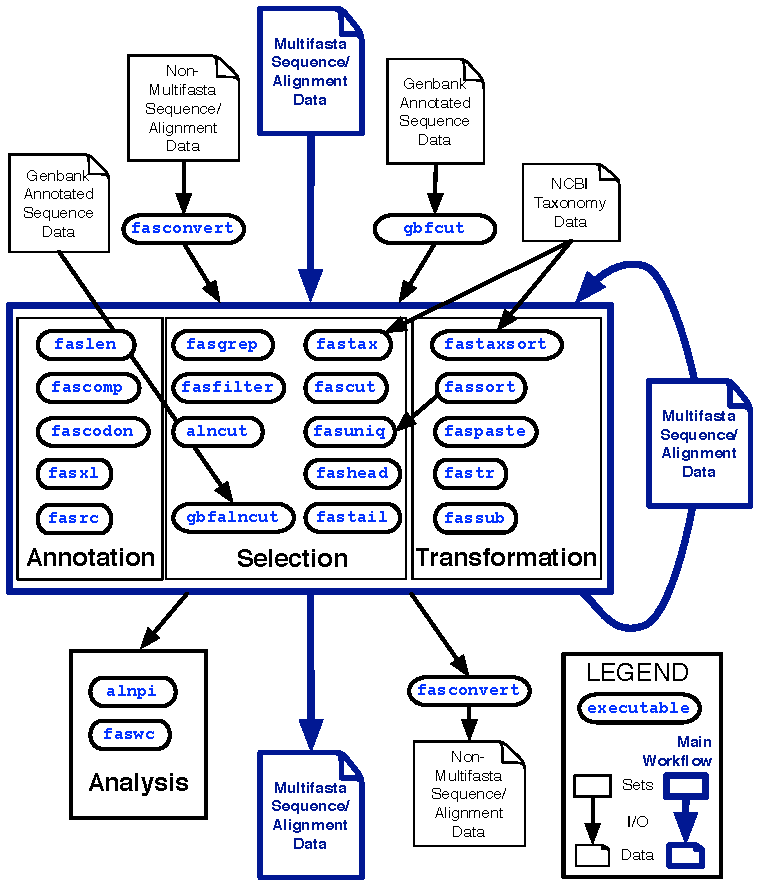
\includegraphics[width=4.5in]{FAST_v8}% This is a *.jpg file
\end{center}
 \textbf{\refstepcounter{figure}\label{fig:01} Figure
   \arabic{figure}.}{ FAST version 1.0 with data and workflow
   dependencies indicated.}
\end{figure}

\begin{figure}
\begin{center}
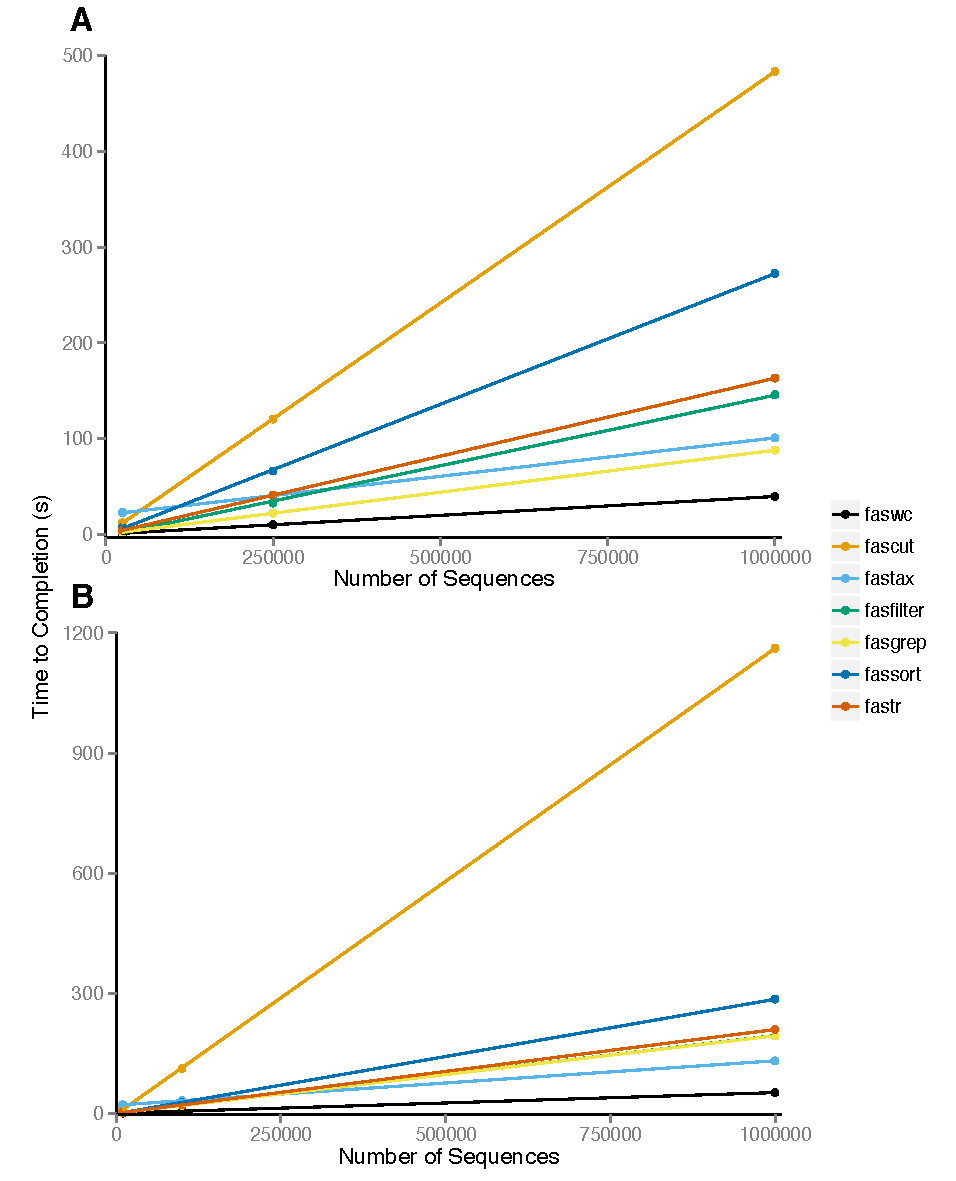
\includegraphics{Figure2}
\end{center}
\textbf{\refstepcounter{figure}\label{fig:02} Figure
  \arabic{figure}.}{ Average processor time of 100 repetitions
  required to complete analysis using indicated utility. Utilities
  were run on six datasets consisting of (a) 25000, 250000, and
  1000000 100bp sequences and (b) 10000, 100000, and 1000000 1000bp
  sequences. }
\end{figure}


\end{document}
